\documentclass[12pt,border=10pt]{standalone}
\usepackage{tikz}
\usetikzlibrary{patterns, calc, arrows.meta, shapes.geometric}
\usepackage{varwidth}

\tikzset{
    sombreado/.style={fill=black!80},
}

\begin{document}

%%% ============================================================
%%% PAGE 1 — NEW Q5: L-tromino rotating around center of 3x3 grid
%%% The difficulty: center cell is ALWAYS shaded (hidden constant),
%%% the L rotates 90° CW each step. Student must see both rules.
%%% ============================================================
\begin{varwidth}{20cm}
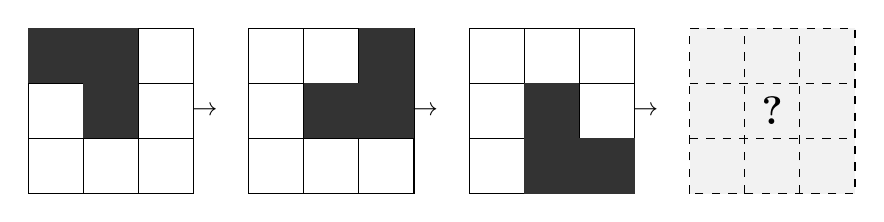
\begin{tikzpicture}[scale=0.7]

% Frame 1: L orientation 0° — center + up + up-left
\begin{scope}[shift={(0,0)}]
\draw (0,0) grid (3,3);
\fill[sombreado] (1,1) rectangle (2,2);  % center (always)
\fill[sombreado] (1,2) rectangle (2,3);  % above center
\fill[sombreado] (0,2) rectangle (1,3);  % top-left
\end{scope}

% Frame 2: L orientation 90° CW — center + right + right-up
\begin{scope}[shift={(4,0)}]
\draw (0,0) grid (3,3);
\fill[sombreado] (1,1) rectangle (2,2);  % center
\fill[sombreado] (2,1) rectangle (3,2);  % right of center
\fill[sombreado] (2,2) rectangle (3,3);  % top-right
\end{scope}

% Frame 3: L orientation 180° — center + down + down-right
\begin{scope}[shift={(8,0)}]
\draw (0,0) grid (3,3);
\fill[sombreado] (1,1) rectangle (2,2);  % center
\fill[sombreado] (1,0) rectangle (2,1);  % below center
\fill[sombreado] (2,0) rectangle (3,1);  % bottom-right
\end{scope}

% Frame 4: ?
\begin{scope}[shift={(12,0)}]
\draw[dashed, fill=gray!10] (0,0) rectangle (3,3);
\draw[dashed] (1,0) -- (1,3);
\draw[dashed] (2,0) -- (2,3);
\draw[dashed] (0,1) -- (3,1);
\draw[dashed] (0,2) -- (3,2);
\node at (1.5,1.5) {\Large\textbf{?}};
\end{scope}

\foreach \x in {3.2, 7.2, 11.2} {
    \node at (\x, 1.5) {\small$\rightarrow$};
}
\end{tikzpicture}

\bigskip

% Options
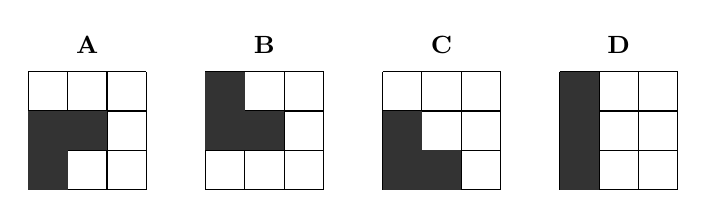
\begin{tikzpicture}[scale=0.5]

% A: CORRECT — L orientation 270° — center + left + left-down
\begin{scope}[shift={(0,0)}]
\node[above] at (1.5,3.2) {\small\textbf{A}};
\draw (0,0) grid (3,3);
\fill[sombreado] (1,1) rectangle (2,2);  % center
\fill[sombreado] (0,1) rectangle (1,2);  % left of center
\fill[sombreado] (0,0) rectangle (1,1);  % bottom-left
\end{scope}

% B: Mirror of correct (left + left-UP instead of left-down)
\begin{scope}[shift={(4.5,0)}]
\node[above] at (1.5,3.2) {\small\textbf{B}};
\draw (0,0) grid (3,3);
\fill[sombreado] (1,1) rectangle (2,2);  % center
\fill[sombreado] (0,1) rectangle (1,2);  % left
\fill[sombreado] (0,2) rectangle (1,3);  % top-left (mirror error)
\end{scope}

% C: No center cell — three cells in bottom-left corner L
\begin{scope}[shift={(9,0)}]
\node[above] at (1.5,3.2) {\small\textbf{C}};
\draw (0,0) grid (3,3);
\fill[sombreado] (0,0) rectangle (1,1);  % bottom-left
\fill[sombreado] (0,1) rectangle (1,2);  % mid-left
\fill[sombreado] (1,0) rectangle (2,1);  % bottom-center
\end{scope}

% D: Correct L orientation BUT shifted to corner (no center cell)
\begin{scope}[shift={(13.5,0)}]
\node[above] at (1.5,3.2) {\small\textbf{D}};
\draw (0,0) grid (3,3);
\fill[sombreado] (0,0) rectangle (1,1);
\fill[sombreado] (0,1) rectangle (1,2);
\fill[sombreado] (0,2) rectangle (1,3);  % entire left column
\end{scope}

\end{tikzpicture}
\end{varwidth}

\newpage

%%% ============================================================
%%% PAGE 2 — NEW Q6: Three independent attributes changing
%%% Rule 1: Shape sides increase (3→4→5→6)
%%% Rule 2: Internal pattern cycles (horiz→vert→diag/→diag\)
%%% Rule 3: Dots below increase (1→2→3→4)
%%% Student must track all three to select correct answer.
%%% ============================================================
\begin{varwidth}{18cm}
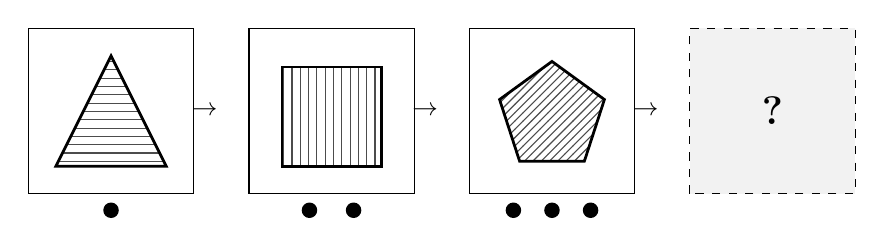
\begin{tikzpicture}[scale=0.7]

% Frame 1: TRIANGLE + horizontal lines + 1 dot
\begin{scope}[shift={(0,0)}]
\draw[line width=0.5pt] (0,0) rectangle (3,3);
\fill[pattern=horizontal lines, pattern color=black!70] (1.5,2.5) -- (0.5,0.5) -- (2.5,0.5) -- cycle;
\draw[line width=1pt] (1.5,2.5) -- (0.5,0.5) -- (2.5,0.5) -- cycle;
\fill (1.5,-0.3) circle (4pt);
\end{scope}

% Frame 2: SQUARE + vertical lines + 2 dots
\begin{scope}[shift={(4,0)}]
\draw[line width=0.5pt] (0,0) rectangle (3,3);
\fill[pattern=vertical lines, pattern color=black!70] (0.6,0.5) rectangle (2.4,2.3);
\draw[line width=1pt] (0.6,0.5) rectangle (2.4,2.3);
\fill (1.1,-0.3) circle (4pt);
\fill (1.9,-0.3) circle (4pt);
\end{scope}

% Frame 3: PENTAGON + NE lines (/) + 3 dots
\begin{scope}[shift={(8,0)}]
\draw[line width=0.5pt] (0,0) rectangle (3,3);
% Pentagon
\fill[pattern=north east lines, pattern color=black!70] 
  ({1.5+1.0*cos(90)},{1.4+1.0*sin(90)}) 
  \foreach \i in {1,...,4} {
    -- ({1.5+1.0*cos(90+\i*72)},{1.4+1.0*sin(90+\i*72)})
  } -- cycle;
\draw[line width=1pt] 
  ({1.5+1.0*cos(90)},{1.4+1.0*sin(90)}) 
  \foreach \i in {1,...,4} {
    -- ({1.5+1.0*cos(90+\i*72)},{1.4+1.0*sin(90+\i*72)})
  } -- cycle;
\fill (0.8,-0.3) circle (4pt);
\fill (1.5,-0.3) circle (4pt);
\fill (2.2,-0.3) circle (4pt);
\end{scope}

% Frame 4: ?
\begin{scope}[shift={(12,0)}]
\draw[dashed, fill=gray!10] (0,0) rectangle (3,3);
\node at (1.5,1.5) {\Large\textbf{?}};
\end{scope}

\foreach \x in {3.2, 7.2, 11.2} {
    \node at (\x, 1.5) {\small$\rightarrow$};
}
\end{tikzpicture}

\bigskip

% Options
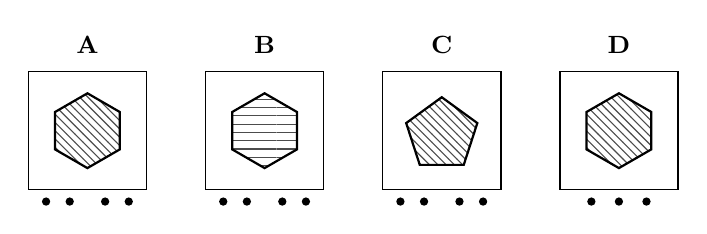
\begin{tikzpicture}[scale=0.5]

% A: CORRECT — Hexagon + NW lines (\) + 4 dots
\begin{scope}[shift={(0,0)}]
\node[above] at (1.5,3.2) {\small\textbf{A}};
\draw[line width=0.5pt] (0,0) rectangle (3,3);
\fill[pattern=north west lines, pattern color=black!70] 
  ({1.5+0.95*cos(30)},{1.5+0.95*sin(30)}) 
  \foreach \i in {1,...,5} {
    -- ({1.5+0.95*cos(30+\i*60)},{1.5+0.95*sin(30+\i*60)})
  } -- cycle;
\draw[line width=0.8pt] 
  ({1.5+0.95*cos(30)},{1.5+0.95*sin(30)}) 
  \foreach \i in {1,...,5} {
    -- ({1.5+0.95*cos(30+\i*60)},{1.5+0.95*sin(30+\i*60)})
  } -- cycle;
\fill (0.45,-0.3) circle (3pt);
\fill (1.05,-0.3) circle (3pt);
\fill (1.95,-0.3) circle (3pt);
\fill (2.55,-0.3) circle (3pt);
\end{scope}

% B: Hexagon + horizontal lines (wrong pattern — reset) + 4 dots
\begin{scope}[shift={(4.5,0)}]
\node[above] at (1.5,3.2) {\small\textbf{B}};
\draw[line width=0.5pt] (0,0) rectangle (3,3);
\fill[pattern=horizontal lines, pattern color=black!70] 
  ({1.5+0.95*cos(30)},{1.5+0.95*sin(30)}) 
  \foreach \i in {1,...,5} {
    -- ({1.5+0.95*cos(30+\i*60)},{1.5+0.95*sin(30+\i*60)})
  } -- cycle;
\draw[line width=0.8pt] 
  ({1.5+0.95*cos(30)},{1.5+0.95*sin(30)}) 
  \foreach \i in {1,...,5} {
    -- ({1.5+0.95*cos(30+\i*60)},{1.5+0.95*sin(30+\i*60)})
  } -- cycle;
\fill (0.45,-0.3) circle (3pt);
\fill (1.05,-0.3) circle (3pt);
\fill (1.95,-0.3) circle (3pt);
\fill (2.55,-0.3) circle (3pt);
\end{scope}

% C: Pentagon (wrong shape — didn't advance) + NW lines + 4 dots
\begin{scope}[shift={(9,0)}]
\node[above] at (1.5,3.2) {\small\textbf{C}};
\draw[line width=0.5pt] (0,0) rectangle (3,3);
\fill[pattern=north west lines, pattern color=black!70] 
  ({1.5+0.95*cos(90)},{1.4+0.95*sin(90)}) 
  \foreach \i in {1,...,4} {
    -- ({1.5+0.95*cos(90+\i*72)},{1.4+0.95*sin(90+\i*72)})
  } -- cycle;
\draw[line width=0.8pt] 
  ({1.5+0.95*cos(90)},{1.4+0.95*sin(90)}) 
  \foreach \i in {1,...,4} {
    -- ({1.5+0.95*cos(90+\i*72)},{1.4+0.95*sin(90+\i*72)})
  } -- cycle;
\fill (0.45,-0.3) circle (3pt);
\fill (1.05,-0.3) circle (3pt);
\fill (1.95,-0.3) circle (3pt);
\fill (2.55,-0.3) circle (3pt);
\end{scope}

% D: Hexagon + NW lines + 3 dots (wrong count)
\begin{scope}[shift={(13.5,0)}]
\node[above] at (1.5,3.2) {\small\textbf{D}};
\draw[line width=0.5pt] (0,0) rectangle (3,3);
\fill[pattern=north west lines, pattern color=black!70] 
  ({1.5+0.95*cos(30)},{1.5+0.95*sin(30)}) 
  \foreach \i in {1,...,5} {
    -- ({1.5+0.95*cos(30+\i*60)},{1.5+0.95*sin(30+\i*60)})
  } -- cycle;
\draw[line width=0.8pt] 
  ({1.5+0.95*cos(30)},{1.5+0.95*sin(30)}) 
  \foreach \i in {1,...,5} {
    -- ({1.5+0.95*cos(30+\i*60)},{1.5+0.95*sin(30+\i*60)})
  } -- cycle;
\fill (0.8,-0.3) circle (3pt);
\fill (1.5,-0.3) circle (3pt);
\fill (2.2,-0.3) circle (3pt);
\end{scope}

\end{tikzpicture}
\end{varwidth}

\end{document}
